\DIFdelbegin %DIFDELCMD < \begin{enumerate}
%DIFDELCMD < \item %%%
\DIFdel{Supplementary Figure~\ref{fig:workflow}
}%DIFDELCMD < \item %%%
\DIFdel{Supplementary Figure~\ref{fig:motclust}
}%DIFDELCMD < \item %%%
\DIFdel{Supplementary Figure~\ref{fig:fitness}
}%DIFDELCMD < \item %%%
\DIFdel{Supplementary Figure~\ref{fig:gresVsOperons}
}%DIFDELCMD < \item %%%
\DIFdel{Supplementary Figure~\ref{fig:corems}
}%DIFDELCMD < \item %%%
\DIFdel{Supplementary Figure~\ref{fig:suppfig6}
}%DIFDELCMD < \end{enumerate}
%DIFDELCMD < 

%DIFDELCMD < \begin{figure}[!b]
%DIFDELCMD < %%%
\DIFdelend \DIFaddbegin \begin{figure}[hp]
\DIFaddendFL \centering
\DIFdelbeginFL %DIFDELCMD < \epsfig{file=figures/e1.eps,width=0.95\linewidth}
%DIFDELCMD < %%%
%DIF < \\\\\vspace{.07in}\hline\\\\\vspace{.07in}
%DIFDELCMD < \caption{{\bf %%%
\DIFdelFL{Detailed workflow for EGRIN 2.0 inference
procedure.}%DIFDELCMD < } %%%
\DIFdelFL{Data input, processing and analysis to construct EGRIN 2.0
model for }%DIFDELCMD < {\it %%%
\DIFdelFL{H. salinarum}%DIFDELCMD < } %%%
\DIFdelFL{and }%DIFDELCMD < {\it %%%
\DIFdelFL{E. coli}%DIFDELCMD < }%%%
\DIFdelFL{, and predictions
generated. Predictions highlighted in individual figures are noted.}%DIFDELCMD < }
%DIFDELCMD < \label{fig:workflow}
%DIFDELCMD < \vspace{-.1in}
%DIFDELCMD < %%%
\DIFdelendFL \DIFaddbeginFL 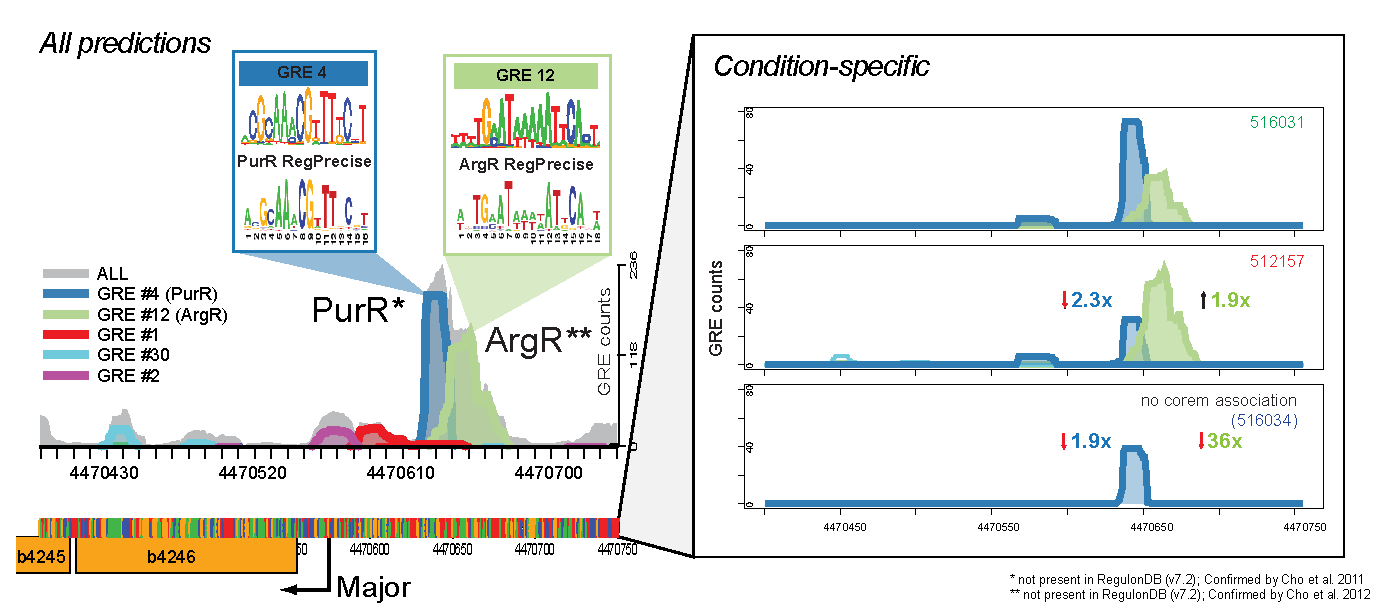
\includegraphics[width=0.95\linewidth]{figures/pyrL.pdf}
\caption[Differential GRE activity in \textit{pyrL} promoter, \textit{E. coli}]{\textbf{\DIFaddFL{Differential GRE activity in }\textit{\DIFaddFL{pyrL}} \DIFaddFL{promoter, }\textit{\DIFaddFL{E. coli}}\DIFaddFL{.}} \DIFaddFL{(Left) Predicted promoter architecture for }{\it \DIFaddFL{E. coli}} \textit{\DIFaddFL{pyrL}} \DIFaddFL{(}\textit{\DIFaddFL{b4246}}\DIFaddFL{). Overlapping GREs matching to PurR (GRE }\#\DIFaddFL{4) and ArgR (GRE }\#\DIFaddFL{12) were detected upstream of pyrL. These sites were not annotated in RegulonDB, but were validated in independent ChIP-chip experiments \mbox{%DIFAUXCMD
\cite{Cho2012,Cho2011a}
}%DIFAUXCMD
. Transcription start site indicated with arrow. (Bottom) Condition-specific promoter architectures for }{\it \DIFaddFL{E. coli}} \textit{\DIFaddFL{pyrL}} \DIFaddFL{(as in Figure 2E). Variation in predicted GRE activity across three different subsets of experimental conditions (counts and fold-change) for two GREs in the }\textit{\DIFaddFL{pyrL}} \DIFaddFL{promoter. Experimental subsets correspond to conditions under which at least one of three nucleotide biosynthetic corems is regulated (denoted by colored names at top-right of each plot)}}
\label{fig:pyrL}
\DIFaddendFL \end{figure}

\DIFdelbegin %DIFDELCMD < \begin{figure}[!b]
%DIFDELCMD < %%%
\DIFdelend \DIFaddbegin \begin{figure}[hp]
\DIFaddendFL \centering
\DIFdelbeginFL %DIFDELCMD < \epsfig{file=figures/e2.eps,width=0.8\linewidth}
%DIFDELCMD < %%%
%DIF < \\\\\vspace{.07in}\hline\\\\\vspace{.07in}
%DIFDELCMD < \caption{{\bf %%%
\DIFdelFL{Genome-wide discovery and validation of gene
regulatory elements (}\DIFdelendFL \DIFaddbeginFL 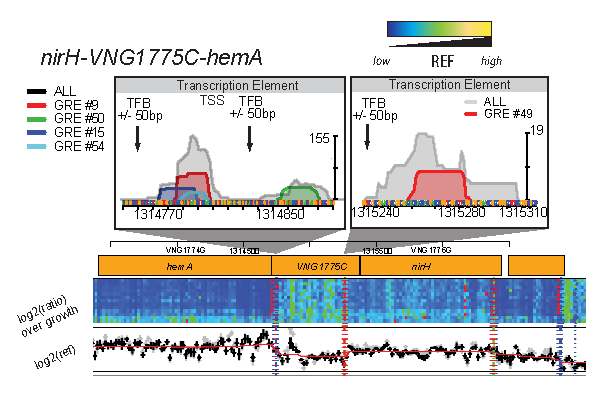
\includegraphics[width=0.95\linewidth]{figures/nirH.pdf}
\caption[GREs regulate multiple transcript isoforms from operons in {\it H. salinarum}, \textit{nirH-VNG1775C-hemA}.]{\textbf{\DIFaddFL{GREs regulate multiple transcript isoforms from operons in }{\it \DIFaddFL{H. salinarum}}\DIFaddFL{, }\textit{\DIFaddFL{nirH-VNG1775C-hemA}}\DIFaddFL{.}} \DIFaddendFL GREs \DIFdelbeginFL \DIFdelFL{). (A) Motif clustering and GRE
identification.}%DIFDELCMD < } %%%
\DIFdelFL{(Left) A schematic of the approach used to align and
cluster individually detected motifs to define GREs. In this example,
similar motifs were aligned and clustered into three GREs using Tomtom
and mcl (Details in Methods and Supplementary Methods). (Center) The
}%DIFDELCMD < {\it %%%
\DIFdelFL{H. salinarum}%DIFDELCMD < } %%%
\DIFdelFL{network of aligned and clustered motifs. (Right)
Two }%DIFDELCMD < {\it %%%
\DIFdelFL{H. salinarum}%DIFDELCMD < } %%%
\DIFdelFL{GREs discovered by this method. The motif logo
of each GRE was generated by summing PSSMs of the individual aligned
motifs in the cluster, as illustrated by three examples of individual
motifs (prior to alignment) for each of the two GREs. Note that
relative to the individual motifs, the averaged GRE motif is more
palindromic - a hallmark of binding sites for dimeric TFs. }%DIFDELCMD < {\bf %%%
\DIFdelFL{(B)
Integration of GRE discovery and Inferelator predictions yields
comprehensive and detailed gene regulatory networks.}%DIFDELCMD < } %%%
\DIFdelFL{EGRIN
2.0-inferred }%DIFDELCMD < {\it %%%
\DIFdelFL{E. coli}%DIFDELCMD < } %%%
\DIFdelFL{regulatory subnetwork for two genes (green
circles) in the PurR/ArgR regulon: carA (b0032) and pyrL (b4246).  The
EGRIN 2.0 predictions are divided into GRE-based (dark violet) and
Inferelator-based (red), and compared to predictions (or annotations)
from other algorithms/databases (yellow: CLR; green: DREAM5 ensemble;
black: RegPrecise; blue: RegulonDB). In two cases
(ArgR$\rightarrow$carA and ArgR$\rightarrow$pyrL), EGRIN 2.0 discovers
regulatory interactions that were missed by either hand-curated
databases or expression-based inference procedures. }%DIFDELCMD < {\bf %%%
\DIFdelFL{(C) Number of TFs
in RegulonDB re-discovered by various methods.}%DIFDELCMD < } %%%
\DIFdelFL{Comparison of EGRIN 2.0
(solid line, far right) to individual }%DIFDELCMD < \cm\ %%%
\DIFdelFL{runs, as well as
multiple runs of k-means, WGCNA, and DISTILLER on subsets of the
expression data. Evaluation made with respect to re-discovery of 88
TFs in RegulonDB with $\geq 3$ unique sites based on genome-wide
binding site locations (FDR $\leq 0.05$). }%DIFDELCMD < {\bf %%%
\DIFdelFL{(D) Genome-wide
distribution of GREs relative to experimentally mapped transcriptional
start sites in }%DIFDELCMD < {\it %%%
\DIFdelFL{H. salinarum}%DIFDELCMD < }%%%
\DIFdelFL{.}%DIFDELCMD < } %%%
\DIFdelFL{(Left) Predicted positions for all GREs
in gene promoters upstream of experimentally mapped transcription
start sites (TSSs; Koide et al., 2009) in and (Right) four example
elements. Distribution peaks for most GREs occur at characteristic
locations. For instance, the location of TATA box-like elements
(GRE }%DIFDELCMD < \#%%%
\DIFdelFL{25) between -21 to -40 nt upstream to TSSs in }%DIFDELCMD < {\it %%%
\DIFdelFL{H. salinarum}%DIFDELCMD < } %%%
\DIFdelFL{is
consistent with the characterized location of basal elements in
archaeal promoters (-25 to 30 nt upstream to TSS). GRE location
enables prediction of putative roles for the cognate TF (}%DIFDELCMD < \eg
%DIFDELCMD < %%%
\DIFdelFL{repressor, activator or a basal factor).}%DIFDELCMD < }
%DIFDELCMD < \label{fig:motclust}
%DIFDELCMD < \vspace{-.1in}
%DIFDELCMD < \end{figure}
%DIFDELCMD < 

%DIFDELCMD < \begin{figure}[!b]
%DIFDELCMD < \centering
%DIFDELCMD < \epsfig{file=figures/e3.eps,width=0.95\linewidth}
%DIFDELCMD < %%%
%DIF < \\\\\vspace{.07in}\hline\\\\\vspace{.07in}
%DIFDELCMD < \caption{{\bf %%%
\DIFdelFL{EGRIN 2.0 models dynamic regulatory mechanisms that
    result in highly correlated fitness effects.}%DIFDELCMD < }  
%DIFDELCMD < {\bf %%%
\DIFdelFL{(A)}%DIFDELCMD < } %%%
\DIFdelFL{(Left) Enrichment for highly correlated, pairwise fitness
  measurements in gene knock outs across 324 conditions before and
  after removing gene associations annotated by operons
  (MicrobesOnline) and regulons (RegulonDB and RegPrecise) (KS-test,
  $D$-statistic). Two-thirds of gene-pairs with most highly correlated
  fitness within corems are not annotated by operons or
  regulons. (Right) Number of genes and associations predicted. }%DIFDELCMD < {\bf %%%
\DIFdelFL{(B)
  Deciphering GREs responsible for regulating corems.}%DIFDELCMD < } %%%
\DIFdelFL{A GRE is
  implicated in regulation of a corem when it is both (1) }\DIFdelendFL located \DIFdelbeginFL \DIFdelFL{within an expanded region (-875nt to +125nt) around the translation
  start site of any gene in the corem; and (2) present in biclusters
  containing a large fraction of corem genes (top decile). Relative
  GRE influence is computed as the frequency with which each GRE was
  discovered in these representative biclusters (see Supplementary
  Methods for more details). Influence scores are illustrated as pie
  charts and reported for each gene individually (}%DIFDELCMD < \eg%%%
\DIFdelFL{, VNG2347G); and
  as a composite by averaging across all genes in a corem. The width
  of each sector in the pie charts is proportional to the frequency of
  GRE discovery.  }%DIFDELCMD < {\bf %%%
\DIFdelFL{(C)}%DIFDELCMD < } %%%
\DIFdelFL{(Top) Predicted promoter architecture for
  }%DIFDELCMD < {\it %%%
\DIFdelFL{E. coli}%DIFDELCMD < } %%%
\DIFdelFL{pyrL (b4246). Overlapping GREs matching to PurR (GRE }%DIFDELCMD < \#%%%
\DIFdelFL{4) and
  ArgR (GRE }%DIFDELCMD < \#%%%
\DIFdelFL{12) were detected upstream of pyrL. These sites were not
  annotated in RegulonDB, but were validated in independent ChIP-chip
  experiments (Cho et al., 2012; Cho et al., 2011). Transcription
  start site indicated with arrow. (Bottom) Condition-specific
  promoter architectures for }%DIFDELCMD < {\it %%%
\DIFdelFL{E. coli}%DIFDELCMD < } %%%
\DIFdelFL{pyrL (as in Figure 2E). Variation
  in predicted GRE activity across three different subsets of
  experimental conditions (counts and fold-change) for two GREs in the
  pyrL promoter. Experimental subsets correspond to conditions under
  which at least one of three nucleotide biosynthetic corems is
  regulated (denoted by colored names at top-right of each plot) }%DIFDELCMD < }
%DIFDELCMD < \label{fig:fitness}
%DIFDELCMD < \vspace{-.1in}
%DIFDELCMD < \end{figure}
%DIFDELCMD < 

%DIFDELCMD < \begin{figure}[!b]
%DIFDELCMD < \centering
%DIFDELCMD < \epsfig{file=figures/e4.eps,width=0.95\linewidth}
%DIFDELCMD < %%%
%DIF < \\\\\vspace{.07in}\hline\\\\\vspace{.07in}
%DIFDELCMD < \caption{{\bf %%%
\DIFdelFL{GREs regulate internal modulation of operons in
    }%DIFDELCMD < {\it %%%
\DIFdelFL{H. salinarum}%DIFDELCMD < }%%%
\DIFdelFL{.}%DIFDELCMD < }  {\bf %%%
\DIFdelFL{(A) GREs located }\DIFdelendFL inside operons coincide with experimentally measured transcriptional break sites. \DIFdelbeginFL %DIFDELCMD < } %%%
\DIFdelendFL Experimentally determined transcription break sites (red dashed lines) above expression profiles of these regions across growth (heatmap, \DIFdelbeginFL \DIFdelFL{Koide
  et al., 2009) }\DIFdelendFL \DIFaddbeginFL \DIFaddFL{\mbox{%DIFAUXCMD
\cite{Koide2009}
}%DIFAUXCMD
}\DIFaddendFL and ChIP-chip TFBs (\DIFdelbeginFL \DIFdelFL{Facciotti et al.}\DIFdelendFL \DIFaddbeginFL \DIFaddFL{\mbox{%DIFAUXCMD
\cite{Facciotti2007}
}%DIFAUXCMD
}\DIFaddendFL , \DIFdelbeginFL \DIFdelFL{2007, }\DIFdelendFL vertical arrows) support the role of GREs in regulating segmentation of the operon in certain conditions. Insets contain regions immediately surrounding transcriptional break sites, including counts of GREs discovered at these locations.\DIFdelbeginFL \DIFdelFL{Three examples of conditionally
  segmented operons are shown. }%DIFDELCMD < {\bf %%%
\DIFdelFL{(B) Alternate regulatory modes for dpp
  operon predicted by corems.}%DIFDELCMD < } %%%
\DIFdelendFL \DIFaddbeginFL }
\label{fig:nirH}
\end{figure}

\begin{figure}[hp]
\centering
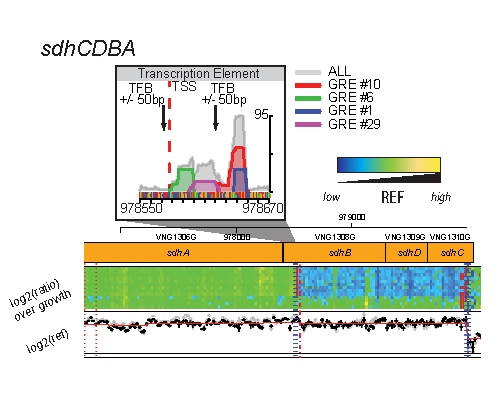
\includegraphics[width=0.95\linewidth]{figures/sdh.pdf}
\caption[GREs regulate multiple transcript isoforms from operons in {\it H. salinarum}, \textit{sdhCDBA}.]{\textbf{\DIFaddFL{GREs regulate multiple transcript isoforms from operons in }{\it \DIFaddFL{H. salinarum}}\DIFaddFL{, }\textit{\DIFaddFL{sdhCDBA}}\DIFaddFL{.}} \DIFaddFL{Caption details included in Figure \ref{fig:nirH}}}
\label{fig:sdh}
\end{figure}

\begin{figure}[hp]
\centering
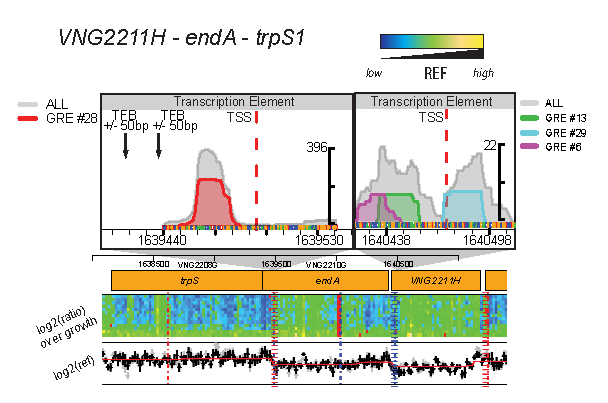
\includegraphics[width=0.95\linewidth]{figures/vng2211h.pdf}
\caption[GREs regulate multiple transcript isoforms from operons in {\it H. salinarum}, \textit{VNG2211H-endA-trpS1}.]{\textbf{\DIFaddFL{GREs regulate multiple transcript isoforms from operons in }{\it \DIFaddFL{H. salinarum}}\DIFaddFL{, }\textit{\DIFaddFL{VNG2211H-endA-trpS1}}\DIFaddFL{.}} \DIFaddFL{Caption details included in Figure \ref{fig:nirH}}}
\label{fig:vng2211h}
\end{figure}

\begin{figure}[hp]
\centering
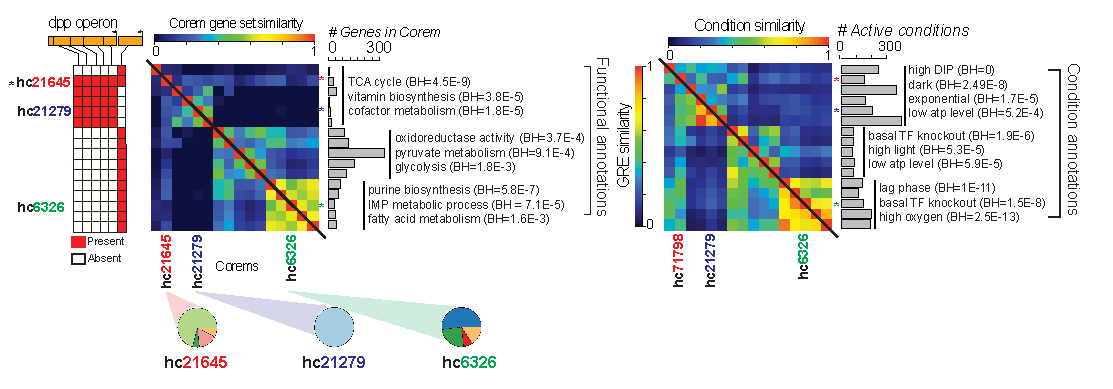
\includegraphics[width=0.95\linewidth]{figures/dpp_heatmaps.pdf}
\caption[Alternate regulatory modes for \textit{dpp} operon predicted by corems]{\textbf{\DIFaddFL{Alternate regulatory modes for }\textit{\DIFaddFL{dpp}} \DIFaddFL{operon predicted by corems.}} \DIFaddendFL Corems group together functionally related sets of genes that are co-regulated in similar environments by similar factors (Left) Presence/absence of \DIFdelbeginFL \DIFdelFL{dpp }\DIFdelendFL \DIFaddbeginFL \textit{\DIFaddFL{dpp}} \DIFaddendFL operon genes in corems. Three classes of corems exist for the dpp operon: (1) the entire operon (\eg hc21645), (2) the leader gene \DIFdelbeginFL \DIFdelFL{dppA
  }\DIFdelendFL \DIFaddbeginFL \textit{\DIFaddFL{dppA}} \DIFaddendFL (\eg hc6326), and (3) five ``tail'' genes excluding \DIFdelbeginFL \DIFdelFL{dppA
  }\DIFdelendFL \DIFaddbeginFL \textit{\DIFaddFL{dppA}} \DIFaddendFL (hc21279). (Middle) Gene similarity between corems (heatmap, Jaccard index). Functional annotations of genes in three highly similar clusters of corems to right. GRE composition for three corems shown below (pie chart, see Figure \DIFdelbeginFL \DIFdelFL{E3B}\DIFdelendFL \DIFaddbeginFL \DIFaddFL{\ref{fig:corem_gres}}\DIFaddendFL ). (Right) Similarity of conditions regulated (heatmap, upper triangle, Jaccard index) and GREs (heatmap, lower triangle, Jaccard index) among corems. Ordering is identical to (Middle). Environmental Ontology term enrichment (see \DIFdelbeginFL \DIFdelFL{Supplemental Methods}\DIFdelendFL \DIFaddbeginFL \DIFaddFL{ref}{}\DIFaddendFL ) for three clusters depicted to right.\DIFdelbeginFL %DIFDELCMD < {\bf %%%
\DIFdelFL{(C) GRE
  compositions coincide with corem membership.}%DIFDELCMD < } %%%
\DIFdelendFL \DIFaddbeginFL }
\label{fig:dpp_heatmaps}
\end{figure}

\begin{figure}[hp]
\centering
\includegraphics[width=0.95\linewidth]{figures/dpp_networks.pdf}
\caption[Network representation of transcriptional isoforms for the \textit{dpp} operon predicted by corems]{\textbf{\DIFaddFL{Network representation of transcriptional isoforms for the }\textit{\DIFaddFL{dpp}} \DIFaddFL{operon predicted by corems.}} \DIFaddendFL Network representation for three corems described \DIFdelbeginFL \DIFdelFL{above}\DIFdelendFL \DIFaddbeginFL \DIFaddFL{in \ref{fig:dpp_heatmaps}}\DIFaddendFL . Genes represented by circles. Edge colors and colored region behind the network indicate corem membership. Pie charts reflect GRE composition of each gene (see Figure \DIFdelbeginFL \DIFdelFL{E3B}\DIFdelendFL \DIFaddbeginFL \DIFaddFL{\ref{fig:corem_gres}}\DIFaddendFL ). Key for pie charts at top. Shading behind nodes (center of network) indicates \DIFdelbeginFL \DIFdelFL{dpp }\DIFdelendFL \DIFaddbeginFL \textit{\DIFaddFL{dpp}} \DIFaddendFL operon genes.\DIFdelbeginFL %DIFDELCMD < {\bf %%%
\DIFdelFL{(D) dppA is more tightly
  co-expressed with genes of hc6326 in some environments than the
  other genes in the dpp operon.}%DIFDELCMD < } %%%
\DIFdelendFL \DIFaddbeginFL }
\label{fig:dpp_networks}
\end{figure}

\begin{figure}[hp]
\centering
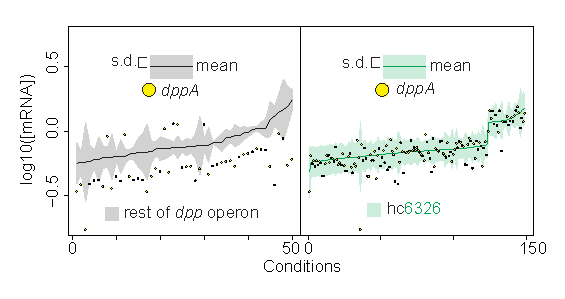
\includegraphics[width=0.95\linewidth]{figures/dpp_expression.pdf}
\caption[\textit{dppA} is more tightly co-expressed with genes of hc6326 in some environments than the other genes in the \textit{dpp} operon]{\textbf{\textit{\DIFaddFL{dppA}} \DIFaddFL{is more tightly co-expressed with genes of hc6326 in some environments than the other genes in the }\textit{\DIFaddFL{dpp}} \DIFaddFL{operon.}} \DIFaddendFL Relative expression of \DIFdelbeginFL \DIFdelFL{dppA }\DIFdelendFL \DIFaddbeginFL \textit{\DIFaddFL{dppA}} \DIFaddendFL compared to (left) other genes of \DIFdelbeginFL \DIFdelFL{dpp }\DIFdelendFL \DIFaddbeginFL \textit{\DIFaddFL{dpp}} \DIFaddendFL opeon and (right) hc6326.\DIFdelbeginFL %DIFDELCMD < {\bf %%%
\DIFdelFL{(E) EGRIN
  2.0 predicts conditional modulation of dpp operon in }%DIFDELCMD < {\it %%%
\DIFdelFL{E. coli}%DIFDELCMD < } %%%
\DIFdelFL{as
  well.}%DIFDELCMD < } %%%
\DIFdelFL{Promoter architecture within intergenic space between dppA and
  dppB suggested locations for TF binding internal to the operon (as
  in }%DIFDELCMD < {\bf %%%
\DIFdelFL{(A)}%DIFDELCMD < }%%%
\DIFdelFL{). GRE binding sites are proximal to an experimentally
  characterized IHF binding site (black horizontal bar; RegulonDB).  }\DIFdelendFL }
\DIFdelbeginFL %DIFDELCMD < \label{fig:gresVsOperons}
%DIFDELCMD < \vspace{-.1in}
%DIFDELCMD < %%%
\DIFdelendFL \DIFaddbeginFL \label{fig:dpp_expression}
\DIFaddendFL \end{figure}

\DIFdelbegin %DIFDELCMD < \begin{figure}[!b]
%DIFDELCMD < %%%
\DIFdelend \DIFaddbegin \begin{figure}[hp]
\DIFaddendFL \centering
\DIFdelbeginFL %DIFDELCMD < \epsfig{file=figures/e5.eps,width=0.95\linewidth}
%DIFDELCMD < %%%
%DIF < \\\\\vspace{.07in}\hline\\\\\vspace{.07in}
%DIFDELCMD < \caption{{\bf %%%
\DIFdelFL{4. Corems integrate and subdivide regulons and operons
    in }%DIFDELCMD < {\it %%%
\DIFdelFL{E. coli}%DIFDELCMD < } %%%
\DIFdelFL{to coordinate related biological processes.}%DIFDELCMD < }  {\bf %%%
\DIFdelFL{(A)
    Corems accurately predict conditionally modulated operons in
    }%DIFDELCMD < {\it %%%
\DIFdelFL{E. coli}%DIFDELCMD < }%%%
\DIFdelFL{.}%DIFDELCMD < } %%%
\DIFdelFL{GREs coincide with experimentally measured break
  sites. Three examples of experimentally determined transcription
  break sites (red dashed lines) in operons predicted by corems to be
  conditionally segmented. Expression levels of these regions were
  profiled across growth in rich media (heatmap). Inset contains
  region immediately surrounding a transcriptional break site,
  including counts of GREs discovered at these locations (as in Figure
  E4A). }%DIFDELCMD < {\bf %%%
\DIFdelFL{(B) Corems model the mechanistic basis for conditional
    subdivision of the PurR regulon.}%DIFDELCMD < } %%%
\DIFdelFL{(Left) Corems identify the most
  highly correlated subgroupings of genes in PurR regulon. Gene
  expression correlation across all experiments (upper triangle)
  compared to similarity of corem membership (lower-triangle, Jaccard
  index) for genes of the PurR regulon (gene identifiers expanded to
  right). (Right) Similarity of regulated conditions (upper triangle,
  Jaccard index) and GREs composition for these genes (bottom
  triangle, Jaccard index). Consistent patterns of
  conditional-activity and GRE composition in their promoter regions
  further supports subdivision of PurR genes into separate
  corems. Gene order is same as left. }%DIFDELCMD < {\bf %%%
\DIFdelFL{(C) Corems reflect
    functional integration across diverse regulatory mechanisms.}%DIFDELCMD < }
%DIFDELCMD <   %%%
\DIFdelFL{Network representation for three of the corems described above (and
  in the text). Genes are represented by circles. Edge colors and
  colored region behind the network indicate corem membership. Pie
  charts reflect GRE composition of each gene (see
  Figure~\ref{fig:fitness}B). Key for pie charts at bottom. GRE-TF
  matches are indicated. Shading behind nodes denotes PurR regulon
  genes. At least 7 different mechanisms regulate the expression of
  these genes.  }%DIFDELCMD < }
%DIFDELCMD < \label{fig:corems}
%DIFDELCMD < \vspace{-.1in}
%DIFDELCMD < %%%
\DIFdelendFL \DIFaddbeginFL 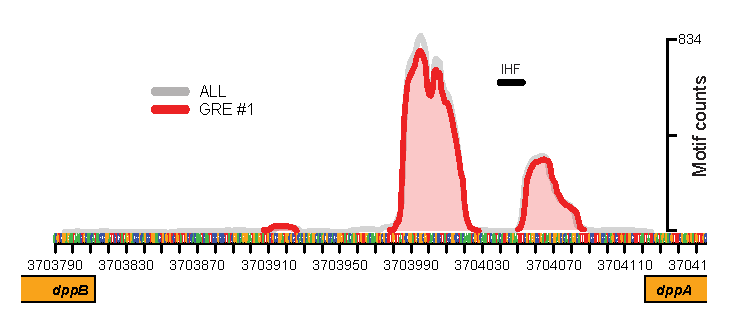
\includegraphics[width=0.95\linewidth]{figures/dpp_ecoli.pdf}
\caption[Evidence for condition-specific transcript isoforms of the \textit{dpp} operon in \textit{E. coli}]{\textbf{\DIFaddFL{Evidence for condition-specific transcript isoforms of the }\textit{\DIFaddFL{dpp}} \DIFaddFL{operon in }\textit{\DIFaddFL{E. coli}}\DIFaddFL{.}} \egrine\DIFaddFL{~predicts conditional modulation of }\textit{\DIFaddFL{dpp}} \DIFaddFL{operon in }{\it \DIFaddFL{E. coli}} \DIFaddFL{as well. Promoter architecture within intergenic space between }\textit{\DIFaddFL{dppA}} \DIFaddFL{and }\textit{\DIFaddFL{dppB}} \DIFaddFL{suggested locations for TF binding internal to the operon (as in Figure 3A). GRE binding sites are proximal to an experimentally characterized IHF binding site (black horizontal bar; RegulonDB).}}
\label{fig:dpp_ecoli}
\DIFaddendFL \end{figure}

\DIFdelbegin %DIFDELCMD < \begin{figure}[!b]
%DIFDELCMD < %%%
\DIFdelend \DIFaddbegin \begin{figure}[hp]
\DIFaddendFL \centering
\DIFdelbeginFL %DIFDELCMD < \epsfig{file=figures/e6.eps,width=0.95\linewidth}
%DIFDELCMD < %%%
%DIF < \\\\\vspace{.07in}\hline\\\\\vspace{.07in}
%DIFDELCMD < \caption{{\bf %%%
\DIFdelFL{Organization of genes in corems provides meaningful link between transcriptional regulation, metabolic dynamics and fitness.}%DIFDELCMD < } 
%DIFDELCMD < {\bf %%%
\DIFdelFL{(A) Genes from corems related to nucleotide biosynthesis have highly
  similar fitness effects when they are deleted.}%DIFDELCMD < } %%%
\DIFdelFL{(Left) Violin plot
  shows distribution of all fitness correlations for genes in three
  nucleotide biosynthesis-associated corems compared to all genes in
  the data set. (Right) KS $D$-Statistic relates to enrichment for
  highly correlated gene-gene fitness associations in the corems. All
  three corems enrich for similar fitness effects (KS FDR $< 5\times 10^{-9}$).
  }%DIFDELCMD < {\bf %%%
\DIFdelFL{(B) Corems model fitness effects that occur in specific
  environments.}%DIFDELCMD < } %%%
\DIFdelFL{Violin plots show distribution of relative fitness
  among corems across conditions (negative values indicate lower
  fitness relative to WT). Brief condition descriptions are displayed
  below. Shading within the violin plot indicates that the
  distribution of fitness values is significantly in that condition
  (KS-test FDR $\leq 0.05$). Fitness values for the subset of genes from
  the PurR regulon that do not occur in ec516031 are displayed to the
  left. These genes do not have significant fitness effects in any of
  the environments tested. Data from (Nichols et al., 2011). }%DIFDELCMD < {\bf %%%
\DIFdelFL{(C)
  Metabolite correlation explains co-regulation within
  metabolically-linked corems.}%DIFDELCMD < } %%%
\DIFdelFL{(Left) Expression correlation for TFs
  associated with three corems described in the text
  (ec516031,ec512157,ec516034). (Right) Correlation allosteric
  regulators for these TFs. TF regulated by each biomolecule listed in
  parentheses (Novichkov et al., 2010). Red boxes indicate PurR-ArgR
  and their corresponding effector molecules. Data from (Ishii et al.,
  2007).
}%DIFDELCMD < }
%DIFDELCMD < \label{fig:suppfig6}
%DIFDELCMD < \vspace{-.1in}
%DIFDELCMD < %%%
\DIFdelendFL \DIFaddbeginFL 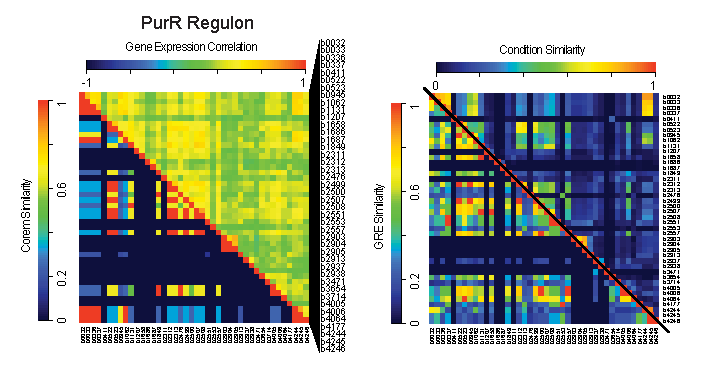
\includegraphics[width=0.95\linewidth]{figures/purR_heatmap.pdf}
\caption[Corems model the mechanistic basis for conditional subdivision of the PurR regulon, \textit{E. coli}]{\textbf{\DIFaddFL{Corems model the mechanistic basis for conditional subdivision of the PurR regulon, }\textit{\DIFaddFL{E. coli}}\DIFaddFL{.}} \DIFaddFL{(Left) Corems identify the most highly correlated subgroupings of genes in PurR regulon. Gene expression correlation across all experiments (upper triangle) compared to similarity of corem membership (lower-triangle, Jaccard index) for genes of the PurR regulon (gene identifiers expanded to right). (Right) Similarity of regulated conditions (upper triangle, Jaccard index) and GREs composition for these genes (bottom triangle, Jaccard index). Consistent patterns of conditional-activity and GRE composition in their promoter regions further supports subdivision of PurR genes into separate corems. Gene order is same as left.}}
\label{fig:purR_heatmap}
\DIFaddendFL \end{figure}
\DIFaddbegin 

\begin{figure}[hp]
\centering
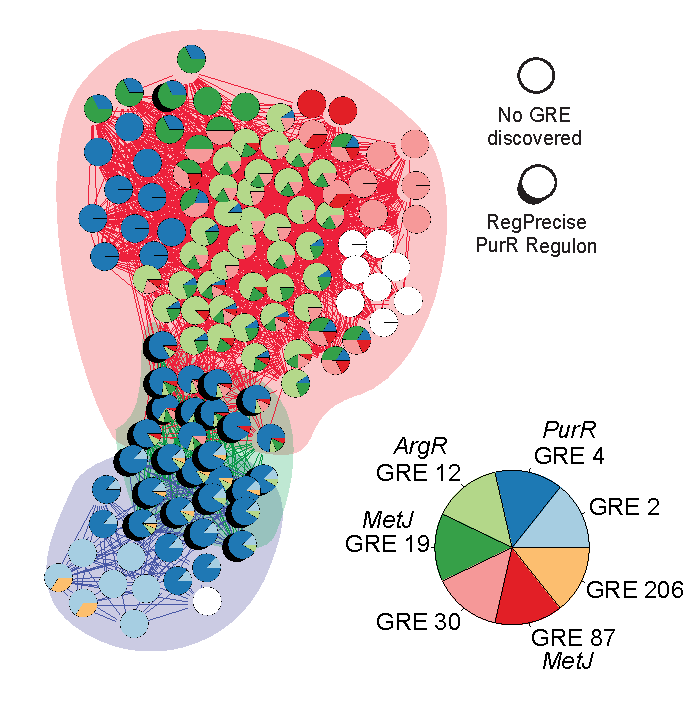
\includegraphics[width=0.95\linewidth]{figures/purR_network.pdf}
\caption[Corems integrate diverse regulatory mechanisms, \textit{E. coli}]{\textbf{\DIFaddFL{Corems integrate diverse regulatory mechanisms, }\textit{\DIFaddFL{E. coli}}\DIFaddFL{.}} \DIFaddFL{Network representation for three corems described in Figure \ref{fig:purR_heatmap}. Genes are represented by circles. Edge colors and colored region behind the network indicate corem membership. Pie charts reflect GRE composition of each gene (see Figure~\ref{fig:corem_gres}). Key for pie charts at bottom. GRE-TF matches are indicated. Shading behind nodes denotes PurR regulon genes. At least 7 different mechanisms regulate the expression of these genes.}}
\label{fig:purR_network}
\end{figure}


\begin{figure}[hp]
\centering
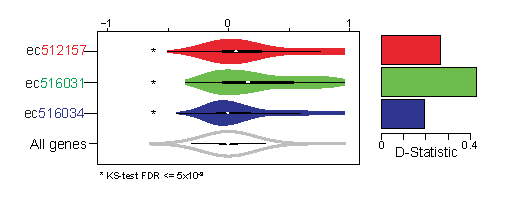
\includegraphics[width=0.95\linewidth]{figures/purR_corem_fitness.pdf}
\caption[Genes from corems related to nucleotide biosynthesis have highly similar fitness effects when they are deleted]{\textbf{\DIFaddFL{Genes from corems related to nucleotide biosynthesis have highly similar fitness effects when they are deleted.}} \DIFaddFL{(Left) Violin plot shows distribution of all fitness correlations for genes in three nucleotide biosynthesis-associated corems compared to all genes in the data set. (Right) KS $D$-Statistic relates to enrichment for highly correlated gene-gene fitness associations in the corems. All three corems enrich for similar fitness effects (KS FDR $< 5\times 10^{-9}$)}}
\label{fig:purR_corem_fitness}
\end{figure}

\begin{figure}[hp]
\centering
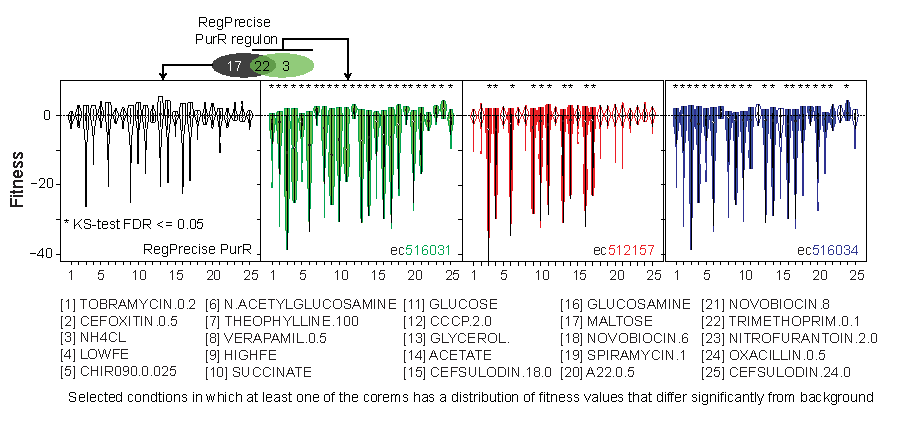
\includegraphics[width=0.95\linewidth]{figures/purR_corem_fitness_specific.pdf}
\caption[Corems model fitness effects that occur in specific environments]{\textbf{\DIFaddFL{Corems model fitness effects that occur in specific environments.}} \DIFaddFL{Violin plots show distribution of relative fitness among corems across conditions (negative values indicate lower fitness relative to WT). Brief condition descriptions are displayed below. Shading within the violin plot indicates that the distribution of fitness values is significantly in that condition (KS-test FDR $\leq 0.05$). Fitness values for the subset of genes from the PurR regulon that do not occur in ec516031 are displayed to the left. These genes do not have significant fitness effects in any of the environments tested. Data from \mbox{%DIFAUXCMD
\cite{Nichols2011}
}%DIFAUXCMD
.}}
\label{fig:purR_corem_fitness_specific}
\end{figure}

\begin{figure}[hp]
\centering
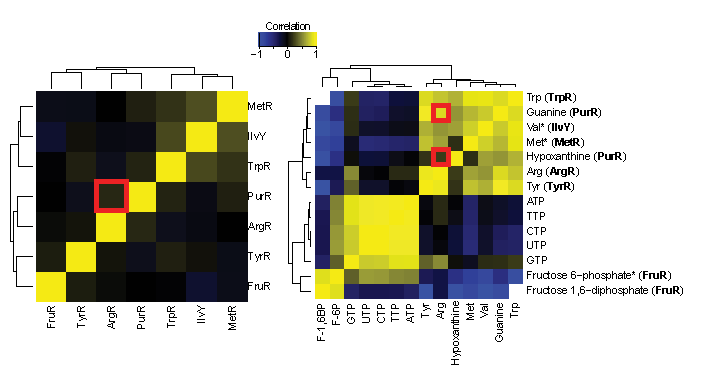
\includegraphics[width=0.95\linewidth]{figures/purR_effector.pdf}
\caption[Metabolite correlations may explain co-regulation within metabolically-linked corems]{\textbf{\DIFaddFL{Metabolite correlations may explain co-regulation within metabolically-linked corems.}} \DIFaddFL{(Left) Expression correlation for TFs associated with three corems described in the text (ec516031,ec512157,ec516034). (Right) Correlation allosteric regulators for these TFs. TF regulated by each biomolecule listed in parentheses \mbox{%DIFAUXCMD
\cite{Novichkov2010}
}%DIFAUXCMD
. Red boxes indicate PurR-ArgR and their corresponding effector molecules. Data from \mbox{%DIFAUXCMD
\cite{Ishii2007}
}%DIFAUXCMD
.}}
\label{fig:purR_effector}
\end{figure}

 \DIFaddend